\documentclass[6pt,letterpaper]{article}
\usepackage[margin=0.25in, top=0.3in, bottom=0.25in]{geometry}
\usepackage{amsmath,amssymb}
\usepackage{multicol}
\usepackage{xcolor}
\usepackage{mdframed}
\usepackage[expansion=false]{microtype}
\usepackage{fancyhdr}
\usepackage{booktabs}
\usepackage{colortbl}
\usepackage{array}
\usepackage{graphicx}

% Colors (match HW1-HW4 cheat sheets)
\definecolor{purple}{HTML}{534AB7}\definecolor{purplebg}{HTML}{EEEDFE}
\definecolor{teal}{HTML}{0F6E56}\definecolor{tealbg}{HTML}{E1F5EE}
\definecolor{coral}{HTML}{993C1D}\definecolor{coralbg}{HTML}{FAECE7}
\definecolor{amber}{HTML}{854F0B}\definecolor{amberbg}{HTML}{FAEEDA}
\definecolor{green}{HTML}{3B6D11}\definecolor{greenbg}{HTML}{EAF3DE}
\definecolor{blue}{HTML}{0C447C}\definecolor{bluebg}{HTML}{E6F1FB}
\definecolor{gray}{HTML}{444441}\definecolor{graybg}{HTML}{F1EFE8}
\definecolor{pink}{HTML}{72243E}\definecolor{pinkbg}{HTML}{FBEAF0}
\definecolor{rowB}{HTML}{F2F2EF}

\newmdenv[linewidth=0.4pt,innerleftmargin=3pt,innerrightmargin=3pt,
  innertopmargin=0.5pt,innerbottommargin=0.5pt,skipabove=0.5pt,skipbelow=0.5pt]{ebox}

\newcommand{\shead}[3]{%
  \noindent\colorbox{#1}{\parbox{\dimexpr\linewidth-2\fboxsep\relax}%
  {\color{#2}\bfseries\fontsize{6}{7}\selectfont #3}}\vspace{0.3pt}}

\newcommand{\eq}[2]{\noindent{\color{gray}\bfseries\fontsize{5.8}{6}\selectfont#1}\enspace{\color{teal}\fontsize{5.5}{6}\selectfont\textit{#2}}}

\setlength{\parindent}{0pt}\setlength{\parskip}{0pt}
\setlength{\columnsep}{5pt}\setlength{\multicolsep}{1pt}

\pagestyle{fancy}\fancyhf{}
\renewcommand{\headrulewidth}{0.3pt}
\fancyhead[L]{\fontsize{6.5}{7}\selectfont\textbf{ECE332 --- Final Cheat Sheet (HW3 + HW4)}}
\fancyhead[R]{\fontsize{6.5}{7}\selectfont Bao Nguyen}

\graphicspath{{../img/}{../../Cheatsheets/Exam1/img/}{../../../Textbook/tables/}}

\begin{document}

%%=============================================================
%% PAGE 1 --- HW3 (BOUNDARIES + WAVEGUIDES)
%%=============================================================
\fontsize{6}{7}\selectfont
\setlength{\abovedisplayskip}{0pt}\setlength{\belowdisplayskip}{0.5pt}
\setlength{\abovedisplayshortskip}{0pt}\setlength{\belowdisplayshortskip}{0pt}
\begin{multicols}{3}

%-- Column 1 -----------------------------------
\shead{purplebg}{purple}{$\tilde{\mathbf{E}}$ PHASOR TEMPLATES (Air: $\varepsilon_r\!=\!\mu_r\!=\!1$)}
\begin{ebox}
\eq{Wavenumber per medium}{nonmag.}
\[k_i = \tfrac{\omega\sqrt{\varepsilon_{r,i}}}{c}\;(\text{rad/m})\quad\Rightarrow\;k_2 = k_1\sqrt{\varepsilon_{r,2}/\varepsilon_{r,1}}\]

\eq{Direction table}{$u\in\{x,y,z\}$ = axis perp.\ to boundary}\\[1pt]
{\centering\makebox[0.98\linewidth][c]{{\setlength{\tabcolsep}{3pt}\begin{tabular}{@{}cccc@{}}
\toprule
Inc dir & Inc & Refl & Trans\\
\midrule
\rowcolor{rowB}$+\hat{u}$ & $e^{-jk_1u}$ & $e^{+jk_1u}$ & $e^{-jk_2u}$\\
$-\hat{u}$ & $e^{+jk_1u}$ & $e^{-jk_1u}$ & $e^{+jk_2u}$\\
\bottomrule
\end{tabular}}}\par}
\textit{$+\hat{u}$ direction $\Leftrightarrow$ Med 2 at $u\!\ge\!0$. Reflected sign flips, transmitted matches incident.}\\[2pt]

\textit{General template (incident has pol.\ $\hat{e}$, amplitude $a_0$):}
\[\begin{aligned}
\tilde{\mathbf{E}}^i &= a_0\hat{e}\,e^{\mp jk_1u}\;\text{(V/m)}&&\text{\tiny (incident wave, Med 1)}\\
\tilde{\mathbf{E}}^r &= \Gamma\,a_0\hat{e}\,e^{\pm jk_1u}\;\text{(V/m)}&&\text{\tiny (reflected wave, Med 1)}\\
\tilde{\mathbf{E}}^t &= \tau\,a_0\hat{e}\,e^{\mp jk_2u}\;\text{(V/m)}&&\text{\tiny (transmitted wave, Med 2)}
\end{aligned}\]
\textit{(lossy med 2: replace $e^{\mp jk_2u}$ with $e^{\mp\alpha_2 u}e^{\mp j\beta_2 u}$)}\\[1pt]
\textit{Total in medium 1: $\tilde{\mathbf{E}}_1 = \tilde{\mathbf{E}}^i + \tilde{\mathbf{E}}^r$.}\\[1pt]
\eq{$\hat{e}$ by polarization}{plug into templates above}
{\centering\makebox[0.98\linewidth][c]{{\setlength{\tabcolsep}{2pt}\begin{tabular}{@{}p{0.30\linewidth}p{0.34\linewidth}p{0.30\linewidth}@{}}
\toprule
Pol. & $\hat{e}$ & Note\\
\midrule
\rowcolor{rowB}Lin.\ $\hat{x}$ & $\hat{x}$ & $E_y=0$\\
Lin.\ $\hat{y}$ & $\hat{y}$ & $E_x=0$\\
\rowcolor{rowB}Lin.\ at $45^\circ$ & $(\hat{x}+\hat{y})/\sqrt{2}$ & in phase\\
RHC & $\hat{x}-j\hat{y}$ & $\delta=-\pi/2$\\
\rowcolor{rowB}LHC & $\hat{x}+j\hat{y}$ & $\delta=+\pi/2$\\
General & $a_x\hat{x}+a_y e^{j\delta}\hat{y}$ & elliptical\\
\bottomrule
\end{tabular}}}\par}
\textit{\color{coral}$\Gamma, \tau$ act on $\hat{e}$ unchanged. Only swap the polarization, not the formulas.}
\end{ebox}

\vspace{1pt}
\shead{bluebg}{blue}{TABLE 8-2 --- $\Gamma, \tau, R, T$ (unitless) SUMMARY}
\begin{ebox}
\textit{\color{coral}\textbf{Med.\ 1} ($z<0$) incident side; \textbf{Med.\ 2} ($z\ge0$) transmitted.}\\[1pt]
{\centering\makebox[0.98\linewidth][c]{{\setlength{\tabcolsep}{0.5pt}\fontsize{4.6}{5.4}\selectfont\begin{tabular}{@{}p{0.205\linewidth}|p{0.13\linewidth}|p{0.32\linewidth}|p{0.325\linewidth}@{}}
\toprule
 & \textbf{Normal} ($\theta_i\!=\!0$) & $\boldsymbol{\perp}$ \textbf{pol} & $\boldsymbol{\parallel}$ \textbf{pol}\\
\midrule
\rowcolor{rowB}$\Gamma$ \tiny refl.\ wav & $\tfrac{\eta_2-\eta_1}{\eta_2+\eta_1}$ & $\tfrac{\eta_2\cos\theta_i-\eta_1\cos\theta_t}{\eta_2\cos\theta_i+\eta_1\cos\theta_t}$ & $\tfrac{\eta_2\cos\theta_t-\eta_1\cos\theta_i}{\eta_2\cos\theta_t+\eta_1\cos\theta_i}$\\
$\tau$ \tiny trans.\ wav & $\tfrac{2\eta_2}{\eta_2+\eta_1}$ & $\tfrac{2\eta_2\cos\theta_i}{\eta_2\cos\theta_i+\eta_1\cos\theta_t}$ & $\tfrac{2\eta_2\cos\theta_i}{\eta_2\cos\theta_t+\eta_1\cos\theta_i}$\\
\rowcolor{rowB}$\tau$ rel.\ & $\tau\!=\!1\!+\!\Gamma$ & $\tau_\perp\!=\!1\!+\!\Gamma_\perp$ & $\tau_\parallel\!=\!(1\!+\!\Gamma_\parallel)\tfrac{\cos\theta_i}{\cos\theta_t}$\\
$R$ \tiny refl.\ pwr & $|\Gamma|^2$ & $|\Gamma_\perp|^2$ & $|\Gamma_\parallel|^2$\\
\rowcolor{rowB}$T$ \tiny trans.\ pwr & $|\tau|^2\tfrac{\eta_1}{\eta_2}$ & $|\tau_\perp|^2\tfrac{\eta_1\cos\theta_t}{\eta_2\cos\theta_i}$ & $|\tau_\parallel|^2\tfrac{\eta_1\cos\theta_t}{\eta_2\cos\theta_i}$\\
$R\!+\!T$ \tiny total & $T\!=\!1\!-\!R$ & $T_\perp\!=\!1\!-\!R_\perp$ & $T_\parallel\!=\!1\!-\!R_\parallel$\\
\bottomrule
\end{tabular}}}\par}
\textit{\color{blue}Notes: $\sin\theta_t\!=\!\sqrt{\mu_1\varepsilon_1/\mu_2\varepsilon_2}\sin\theta_i$;\ nonmag.\ $\Rightarrow\eta_2/\eta_1\!=\!n_1/n_2$.}\\[2pt]

\eq{Intrinsic impedance $\eta_i$}{plug into table above}
\[\eta_i = \sqrt{\tfrac{\mu_r}{\varepsilon_r}}\,\eta_0 \xrightarrow{\mu_r=1} \tfrac{\eta_0}{\sqrt{\varepsilon_{r,i}}}\;(\Omega)\qquad \eta_0=120\pi\!\approx\!377\,\Omega\]
\textit{\color{coral}Default $\mu_r=1$ (air, dielectric). Use $\mu_r\!\ne\!1$ only if problem says ``ferromagnetic''/iron/ferrite/etc.}

\eq{Low-loss correction $\eta_c$}{$\sigma/(\omega\varepsilon)\ll1$}
\[\eta_c \approx \sqrt{\tfrac{\mu}{\varepsilon'}}\!\left(1+j\tfrac{\sigma}{2\omega\varepsilon'}\right) \xrightarrow{\text{drop }j}\; \tfrac{\eta_0}{\sqrt{\varepsilon_r}}\]
\textit{\color{coral}For $\Gamma$/$\tau$ just use $\eta_0/\sqrt{\varepsilon_r}$. The $j$ term is for $|\eta_c|, \theta_\eta$. See LOSSY MEDIA --- 5 CASES.}
\end{ebox}

\vspace{1pt}
\shead{coralbg}{coral}{POWER REFLECTION \& TRANSMISSION}
\begin{ebox}
\eq{\% reflected}{always}\,$\%P_r = 100\,|\Gamma|^2$\\
\eq{\% transmitted}{$\eta$-ratio matters!}\,$\%P_t = 100\,|\tau|^2\,\eta_1/\eta_2$\\
\textit{Check: $\%P_r + \%P_t = 100$.}
\end{ebox}

\columnbreak

%-- Column 2 -----------------------------------
\shead{tealbg}{teal}{SNELL'S LAW --- OBLIQUE INCIDENCE}
\begin{ebox}
\eq{Single boundary}{angles from normal}
\[\sin\theta_2 = \sin\theta_1\sqrt{\tfrac{\varepsilon_{r1}}{\varepsilon_{r2}}} = \sin\theta_1\,\tfrac{n_1}{n_2}\]

\eq{Multilayer chain}{stack of slabs $1\to2\to3\to4$}
\[\sin\theta_{i+1} = \sin\theta_i\sqrt{\tfrac{\varepsilon_{r,i}}{\varepsilon_{r,i+1}}}\]

\eq{Air--slabs--air shortcut}{outer media identical}
\[\theta_{\text{exit}} = \theta_{\text{incident}}\]
\textit{\color{coral}Snell only sets angles. Reflection/transmission \emph{magnitudes} need Fresnel coefficients (parallel vs perpendicular).}
\end{ebox}

\vspace{1pt}
\shead{tealbg}{teal}{LATERAL DISPLACEMENT}
\begin{ebox}
\begin{center}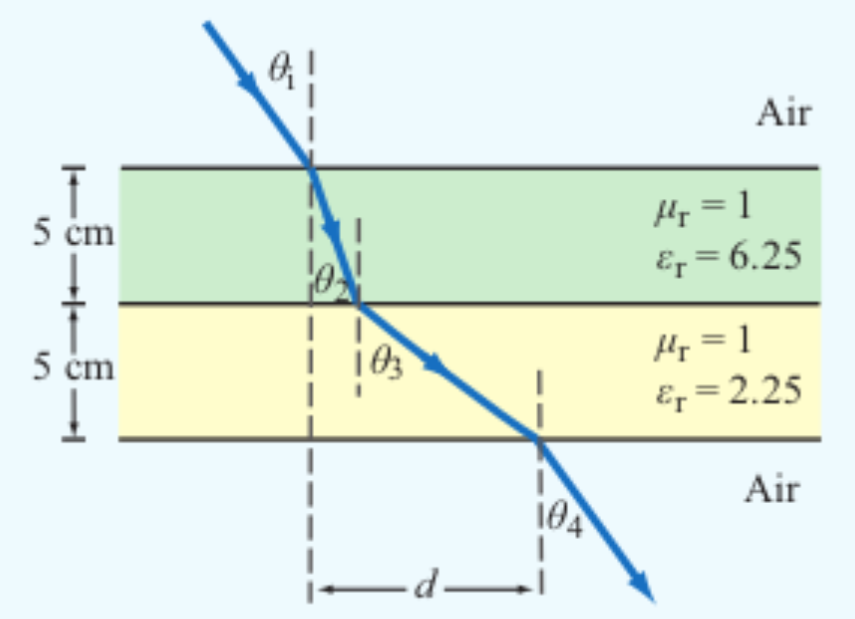
\includegraphics[width=0.65\linewidth]{p3_layered_diagram}\end{center}
\eq{Beam offset through $N$ slabs}{thickness $t_i$, refracted angle inside slab $i$}
\eq{Slab-indexed}{$\theta_i = $ angle inside slab $i$;\ $t_i = $ slab thickness (m)}
\[d = \sum_{i=1}^{N} t_i\,\tan\theta_i\]
\textit{The angle ($\theta_i$) in the formula is always the one the ray makes \emph{inside that slab of height ($t_i$)}.}
\end{ebox}

\vspace{1pt}
\shead{coralbg}{coral}{LOSSY MEDIA --- 5 CASES}
\begin{ebox}
\eq{Loss tangent}{$\varepsilon'\!=\!\varepsilon_r\varepsilon_0$;\, $\varepsilon_0\!=\!8.854\!\times\!10^{-12}$ F/m}
\[\tfrac{\varepsilon''}{\varepsilon'} = \tfrac{\sigma}{\omega\varepsilon_r\varepsilon_0}\]

{\centering\makebox[0.98\linewidth][c]{{\setlength{\tabcolsep}{2pt}\fontsize{5.6}{6.5}\selectfont\begin{tabular}{@{}p{0.28\linewidth}p{0.22\linewidth}p{0.43\linewidth}@{}}
\toprule
Type & $\sigma/\omega\varepsilon$ & $\eta_c,\;\alpha,\;\beta$\\
\midrule
\rowcolor{rowB}Lossless ($\sigma\!=\!0$) & 0 & $\eta\!=\!\eta_0/\sqrt{\varepsilon_r}$ exact\newline $\alpha\!=\!0$,\;$\beta\!=\!\omega\sqrt{\varepsilon_r}/c$\\
Low-loss & $<10^{-2}$ & $\eta_c\!\approx\!\tfrac{\eta_0}{\sqrt{\varepsilon_r}}\!\left(1{+}j\tfrac{\sigma}{2\omega\varepsilon'}\right)$\newline $\alpha\!\approx\!\tfrac{\sigma\eta_0}{2\sqrt{\varepsilon_r}}$,\;$\beta\!\approx\!\tfrac{\omega\sqrt{\varepsilon_r}}{c}$\\
\rowcolor{rowB}Quasi-cond. & $10^{-2}$--$10^2$ & exact: $(\eta/\sqrt{X})e^{j\theta_\eta}$\newline see below\\
Good cond. & $>10^2$ & $\eta_c\!\approx\!(1{+}j)\sqrt{\pi f\mu/\sigma}$\newline $\alpha\!\approx\!\beta\!\approx\!\sqrt{\pi f\mu\sigma}$\\
\rowcolor{rowB}Magnetic & any & keep full $\sqrt{\mu_r/\varepsilon_r}\,\eta_0$\\
\bottomrule
\end{tabular}}}\par}
\textit{\color{coral}For $\Gamma/\tau$: drop $j$ correction; use $\eta_0/\sqrt{\varepsilon_r}$. Magnetic: keep $\mu_r$.}

\eq{Low-loss quick params}{$\sigma/(\omega\varepsilon)\!\ll\!1$, $\mu_r\!=\!1$}
\[\alpha\!\approx\!\tfrac{\sigma\eta_0}{2\sqrt{\varepsilon_r}}\,\text{(Np/m)},\;\beta\!\approx\!\tfrac{\omega\sqrt{\varepsilon_r}}{c}\,\text{(rad/m)},\;\eta_c\!\approx\!\tfrac{\eta_0}{\sqrt{\varepsilon_r}}\,(\Omega)\]

\eq{Exact (quasi-cond)}{$X=\sqrt{1+(\varepsilon''/\varepsilon')^2}$}
\[\alpha=\omega\sqrt{\tfrac{\mu\varepsilon'}{2}}\sqrt{X{-}1},\;\;\beta=\omega\sqrt{\tfrac{\mu\varepsilon'}{2}}\sqrt{X{+}1}\]
\[\theta_\eta = \tfrac{1}{2}\arctan\!\tfrac{\sigma}{\omega\varepsilon'}\]
\end{ebox}

\columnbreak

%-- Column 3 -----------------------------------
\shead{coralbg}{coral}{RECTANGULAR WAVEGUIDE --- MODES}
\begin{ebox}
\eq{TE mode}{$E_z=0$, $H_z\ne0$}\,\eq{TM mode}{$H_z=0$, $E_z\ne0$}\\[1pt]
\textit{Dimensions $a\times b$ with $a>b$ along $\hat{x},\hat{y}$; wave in $\hat{z}$.}\\[1pt]
\eq{$E_x$ form (TE)}{read $m,n$ from arguments}
\[E_x \propto \cos\!\left(\tfrac{m\pi x}{a}\right)\sin\!\left(\tfrac{n\pi y}{b}\right)\sin(\omega t-\beta z)\]
\textit{coef.\ on $x$ = $m\pi/a$; coef.\ on $y$ = $n\pi/b$.}\\[1pt]

\eq{Identify TE$_{mn}$ vs TM$_{mn}$}{cos/sin pattern of $E_x$ is identical for both!}\\
1.\ Read the problem statement (e.g.\ ``a TE wave''~$\to$ TE).\\
2.\ If $m\!=\!0$ or $n\!=\!0$ in the mode label\ $\Rightarrow$ must be TE (TM forbids 0).\\
3.\ Source field $H_z(x,y)$ given $\Rightarrow$ TE.\ Source field $E_z(x,y)$ given $\Rightarrow$ TM.\\[1pt]
\textit{\color{coral}TE allows at least one of $m,n\!\ge\!1$ (other can be 0). TM needs both $m,n\!\ge\!1$. So TE$_{10}$ exists but TM$_{10}$ doesn't.}
\end{ebox}

\vspace{1pt}
\shead{coralbg}{coral}{TABLE 8-3 --- FULL FIELD COMPONENTS}
\begin{ebox}
\textit{$e^{-j\beta z}$ factor omitted. $k_c^2\!=\!(m\pi/a)^2\!+\!(n\pi/b)^2$. $\tilde{E}$ in V/m, $\tilde{H}$ in A/m, $Z$ in $\Omega$.}\\[1pt]

\eq{TE mode}{generator: $\tilde{H}_z$}
\[\tilde{H}_z = H_0\cos\!\tfrac{m\pi x}{a}\cos\!\tfrac{n\pi y}{b}\]
\[\tilde{E}_x = \tfrac{j\omega\mu}{k_c^2}\!\left(\tfrac{n\pi}{b}\right) H_0\cos\!\tfrac{m\pi x}{a}\sin\!\tfrac{n\pi y}{b}\]
\[\tilde{E}_y = -\tfrac{j\omega\mu}{k_c^2}\!\left(\tfrac{m\pi}{a}\right) H_0\sin\!\tfrac{m\pi x}{a}\cos\!\tfrac{n\pi y}{b}\]
\[\tilde{E}_z = 0,\;\; \tilde{H}_x = -\tilde{E}_y/Z_\text{TE},\;\; \tilde{H}_y = \tilde{E}_x/Z_\text{TE}\]
\[Z_\text{TE} = \eta/\sqrt{1-(f_c/f)^2}\]

\eq{TM mode}{generator: $\tilde{E}_z$}
\[\tilde{E}_z = E_0\sin\!\tfrac{m\pi x}{a}\sin\!\tfrac{n\pi y}{b}\]
\[\tilde{E}_x = -\tfrac{j\beta}{k_c^2}\!\left(\tfrac{m\pi}{a}\right) E_0\cos\!\tfrac{m\pi x}{a}\sin\!\tfrac{n\pi y}{b}\]
\[\tilde{E}_y = -\tfrac{j\beta}{k_c^2}\!\left(\tfrac{n\pi}{b}\right) E_0\sin\!\tfrac{m\pi x}{a}\cos\!\tfrac{n\pi y}{b}\]
\[\tilde{H}_z = 0,\;\; \tilde{H}_x = -\tilde{E}_y/Z_\text{TM},\;\; \tilde{H}_y = \tilde{E}_x/Z_\text{TM}\]
\[Z_\text{TM} = \eta\sqrt{1-(f_c/f)^2}\]

\eq{TEM plane wave}{for reference}
\[\tilde{E}_x = E_0\,e^{-j\beta z},\;\; \tilde{H}_y = \tilde{E}_x/\eta\]
\[\eta = \sqrt{\mu/\varepsilon}\;(\Omega),\;\; f_c\text{ N/A},\;\; k = \omega\sqrt{\mu\varepsilon}\]

\eq{Properties common to TE/TM}{}
\[f_c = \tfrac{u_{p0}}{2}\sqrt{(m/a)^2+(n/b)^2}\;(\text{Hz})\]
\[\beta = k\sqrt{1-(f_c/f)^2}\;(\text{rad/m})\]
\[u_p = \tfrac{\omega}{\beta} = \tfrac{u_{p0}}{\sqrt{1-(f_c/f)^2}}\;(\text{m/s})\]
\end{ebox}

\vspace{1pt}
\shead{coralbg}{coral}{CUTOFF FREQUENCY}
\begin{ebox}
\eq{Common cutoffs ($a>b$)}{$f_c$ formula in Table 8-3}\\
{\centering\makebox[0.98\linewidth][c]{{\setlength{\tabcolsep}{2pt}\begin{tabular}{@{}p{0.22\linewidth}p{0.70\linewidth}@{}}
\toprule
Mode & $f_{mn}$\\
\midrule
\rowcolor{rowB}$u_{p0}$ & $c/\sqrt{\varepsilon_r}$ (hollow: $u_{p0}=c$)\\
TE$_{10}$ & $f_{10}=u_{p0}/(2a)$ (dominant)\\
\rowcolor{rowB}TE$_{01}$ & $f_{01}=u_{p0}/(2b)$\\
TE$_{20}$ & $f_{20}=u_{p0}/a = 2f_{10}$\\
\rowcolor{rowB}TE$_{11}$,TM$_{11}$ & $f_{11}=\tfrac{u_{p0}}{2}\sqrt{1/a^2+1/b^2}$\\
\bottomrule
\end{tabular}}}\par}
\textit{Propagation requires $f>f_{mn}$. In $Z_\text{TE}$/$Z_\text{TM}$ and $u_g$, $f_c=f_{mn}$ of the excited mode.}
\end{ebox}

\vspace{1pt}
\shead{coralbg}{coral}{$\varepsilon_r$ FROM DISPERSION}
\begin{ebox}
\eq{Given $\omega$, $\beta$, mode $(m,n)$}{result is unitless}
\[\varepsilon_r = \tfrac{c^2}{\omega^2}\!\left[\beta^2 + \!\left(\tfrac{m\pi}{a}\right)^{\!2}\!+\!\left(\tfrac{n\pi}{b}\right)^{\!2}\right]\;(\text{unitless})\]
\textit{Inputs: $\omega$ (rad/s), $\beta$ (rad/m), $a,b$ (m), $c=3\!\times\!10^8$ (m/s), $m,n$ (unitless).}
\end{ebox}

\vspace{1pt}
\shead{amberbg}{amber}{GROUP VELOCITY \& TRAVEL TIME}
\begin{ebox}
\[u_g = u_{p0}\sqrt{1-(f_{mn}/f)^2}\;\text{(m/s)},\quad u_p u_g = u_{p0}^2\]
\[t = L/u_g\;\text{(s)}\quad\text{travel time through guide of length }L\]
\textit{Higher modes have lower $u_g$ $\Rightarrow$ arrive later.}
\end{ebox}

\end{multicols}

% Bottom strip page 1
\vfill
\vspace{1pt}
\noindent
\begin{minipage}[t]{0.19\linewidth}
\shead{purplebg}{purple}{BOUNDARY}
\begin{ebox}
$\eta_1,\eta_2$ --- imp.\ ($\Omega$)\\
$\Gamma,\tau,R,T$ --- coeffs (unitless)\\
$\tau\!=\!1\!+\!\Gamma$;\ $R\!=\!|\Gamma|^2$\\
$k_i\!=\!\omega\sqrt{\varepsilon_{r,i}}/c$ (rad/m)\\
$\alpha_2$ (Np/m), $\beta_2$ (rad/m): lossy\\
$z\!=\!0$ --- boundary plane (m)\\
$\eta_0\!=\!120\pi\!\approx\!377\,\Omega$
\end{ebox}
\end{minipage}\hfill
\begin{minipage}[t]{0.19\linewidth}
\shead{tealbg}{teal}{SNELL / OBLIQUE}
\begin{ebox}
$\theta_i,\theta_t$ --- angles from normal\\
$n_i=\sqrt{\varepsilon_{r,i}}$ --- index of refr.\\
$t_i$ --- slab thickness (m)\\
$d$ --- lateral disp.\ (m)\\
plane of inc.\ = plane of $\hat{k}$+normal\\
$\perp$: $\mathbf{E}\perp$ this plane\\
$\parallel$: $\mathbf{E}\parallel$ this plane
\end{ebox}
\end{minipage}\hfill
\begin{minipage}[t]{0.19\linewidth}
\shead{coralbg}{coral}{WAVEGUIDE}
\begin{ebox}
$a,b$ --- wide, narrow dim.\ (m); $a>b$\\
$m,n$ --- mode indices (int.)\\
$f_{mn}$ --- cutoff (Hz)\\
$\beta$ --- prop.\ const (rad/m)\\
$Z_{\text{TE/TM}}$ --- wave imp.\ ($\Omega$)\\
$E_x$ --- E-field comp.\ (V/m)\\
$H_y$ --- H-field comp.\ (A/m)\\
$\eta=\eta_0/\sqrt{\varepsilon_r}$
\end{ebox}
\end{minipage}\hfill
\begin{minipage}[t]{0.19\linewidth}
\shead{amberbg}{amber}{VELOCITIES}
\begin{ebox}
$u_{p0}=c/\sqrt{\varepsilon_r}$ --- bulk phase vel.\\
$u_p=u_{p0}/\sqrt{1-(f_c/f)^2}$\\
$u_g=u_{p0}\sqrt{1-(f_c/f)^2}$\\
$u_p u_g = u_{p0}^2$\\
$t=L/u_g$ --- travel time\\
$c=3\times10^8$ m/s
\end{ebox}
\end{minipage}\hfill
\begin{minipage}[t]{0.19\linewidth}
\shead{graybg}{gray}{POWER \& UNITS}
\begin{ebox}
$\%P_r,\%P_t$ --- pwr refl./trans.\ (unitless)\\
$\%P_r\!=\!100|\Gamma|^2$\\
$\%P_t\!=\!100|\tau|^2\eta_1/\eta_2$\\
$\%P_r+\%P_t=100$\\
$\sigma$ (S/m), $\varepsilon$ (F/m), $\mu$ (H/m)\\
$\varepsilon_0\!=\!8.85\!\times\!10^{-12}$ F/m\\
$\mu_0\!=\!4\pi\!\times\!10^{-7}$ H/m
\end{ebox}
\end{minipage}

\newpage

%%=============================================================
%% PAGE 2 --- HW4 (ANTENNAS + FRIIS + ARRAYS)
%%=============================================================
\fontsize{6}{7}\selectfont
\setlength{\abovedisplayskip}{0pt}\setlength{\belowdisplayskip}{0.5pt}
\setlength{\abovedisplayshortskip}{0pt}\setlength{\belowdisplayshortskip}{0pt}
\begin{multicols}{3}

%-- Column 1 -----------------------------------
\shead{purplebg}{purple}{DIPOLE TYPE BY LENGTH}
\begin{ebox}
\eq{STEP 0 --- always start here}{$\lambda$ = wavelength (m), $l$ = antenna rod length (m), $c\!=\!3\!\times\!10^8$ m/s}
\[\boxed{\lambda = \tfrac{c}{f}\;(\text{m})}\qquad\text{ratio } \tfrac{l}{\lambda}\to\text{ pick row below}\]
{\centering\makebox[0.98\linewidth][c]{{\setlength{\tabcolsep}{2pt}\begin{tabular}{@{}p{0.22\linewidth}p{0.32\linewidth}p{0.38\linewidth}@{}}
\toprule
$l/\lambda$ & Type & Use formula\\
\midrule
\rowcolor{rowB}$<1/50$ & Hertzian (short) & HERTZIAN $S(R,\theta)$, $D\!=\!1.5$\\
$=1/4$ & Quarter-wave & ARB formula, $\pi l/\lambda\!=\!\pi/4$\\
\rowcolor{rowB}$=1/2$ & Half-wave & half-wave shortcut, $D\!=\!1.64$, $R_{\text{rad}}\!=\!73\,\Omega$\\
$=1$ & Full-wave & ARB, $D\!=\!2.41$, $R_{\text{rad}}\!=\!199\,\Omega$\\
\rowcolor{rowB}other & Arbitrary & ARB formula\\
\bottomrule
\end{tabular}}}\par}
\textit{\color{coral}If $l/\lambda<1/50$ STOP and use Hertzian. Do NOT plug small $l$ into the arbitrary formula --- wrong shape.}
\end{ebox}

\vspace{1pt}
\shead{purplebg}{purple}{HERTZIAN DIPOLE --- $S(R,\theta)$}
\begin{ebox}
\eq{Far-field E,H phasors}{small $l\!\ll\!\lambda$}
\[\tilde{E}_\theta = \tfrac{j I_0 k l \eta_0}{4\pi}\tfrac{e^{-jkR}}{R}\sin\theta,\;\; \tilde{H}_\phi = \tilde{E}_\theta/\eta_0\]
\eq{Power density}{$l/\lambda<1/50$; far field}
\[S(R,\theta) = \tfrac{\eta_0 k^2 I_0^2 l^2}{32\pi^2 R^2}\sin^2\theta = S_{\max}\sin^2\theta\,(\text{W/m}^2)\]
\textit{$l$ rod length (m); $I_0$ peak current (A); $R$ obs.\ dist.\ (m); $\theta$ from dipole axis; $k\!=\!2\pi/\lambda$ (rad/m); $\eta_0\!=\!120\pi\!\approx\!377\,\Omega$; $S_{\max}$ = max pwr density (the prefactor).}\\
\eq{Max @ broadside}{$\perp$ to dipole axis = equator plane}\,$\theta_{\max}\!=\!\pi/2$;\, \eq{$D$}{exact}\,$D\!=\!1.5$ (1.76 dB)\\
\eq{Total radiated power}{}\,$P_{\text{rad}}\!=\!\tfrac{\eta_0\pi}{3}(I_0 l/\lambda)^2$\,(W)
\end{ebox}

\vspace{1pt}
\shead{tealbg}{teal}{ARBITRARY-LENGTH DIPOLE --- $S(\theta)$}
\begin{ebox}
\eq{Power density at $R$}{any $l$}
\[S(\theta) = \tfrac{15 I_0^2}{\pi R^2}\!\left[\tfrac{\cos\!\left(\tfrac{\pi l}{\lambda}\cos\theta\right)-\cos\!\left(\tfrac{\pi l}{\lambda}\right)}{\sin\theta}\right]^{\!2}\]
\textit{\color{coral}At $\theta\!=\!0,\pi$: bracket is $0/0$. L'H\^opital $\Rightarrow$ $S\!=\!0$ (no axial radiation). TI-36X Pro alt: evaluate bracket at $\theta\!=\!0.001$ rad $\to$ tiny $\to 0$.}\\[1pt]
\eq{Normalized pattern}{dimensionless}\ \ $F(\theta)\!=\!S(\theta)/S_{\max}$
\end{ebox}

\vspace{1pt}
\shead{graybg}{gray}{COMMON ANGLES (deg $\leftrightarrow$ rad, trig values)}
\begin{ebox}
\eq{Conversion}{multiply by $\pi/180$ or $180/\pi$}
\[\theta_{\text{rad}} = \theta_{\text{deg}}\cdot\tfrac{\pi}{180}\qquad \theta_{\text{deg}} = \theta_{\text{rad}}\cdot\tfrac{180}{\pi}\]
{\centering\makebox[0.98\linewidth][c]{{\setlength{\tabcolsep}{2pt}\begin{tabular}{@{}cccccc@{}}
\toprule
$^\circ$ & rad & $\sin\theta$ & $\cos\theta$ & $\sin^2\theta$ & $\cos^2\theta$\\
\midrule
\rowcolor{rowB}0   & 0       & 0          & 1          & 0   & 1\\
30  & $\pi/6$ & $1/2$      & $\sqrt{3}/2$ & $1/4$ & $3/4$\\
\rowcolor{rowB}45  & $\pi/4$ & $\sqrt{2}/2$ & $\sqrt{2}/2$ & $1/2$ & $1/2$\\
60  & $\pi/3$ & $\sqrt{3}/2$ & $1/2$      & $3/4$ & $1/4$\\
\rowcolor{rowB}90  & $\pi/2$ & 1          & 0          & 1   & 0\\
180 & $\pi$   & 0          & $-1$       & 0   & 1\\
\bottomrule
\end{tabular}}}\par}
\textit{Antenna formulas usually take $\theta$ in rad. RAD mode on calc.}
\end{ebox}

\vspace{1pt}
\shead{pinkbg}{pink}{LINEAR ANTENNA ARRAY}
\begin{ebox}
\textit{$N$ identical elements along axis, spacing $d$, equal phase (broadside, $\theta_\text{max}\!=\!\pi/2$). Total pattern $S\!=\!S_e\!\cdot\!F_a$ ($S_e$ = single elem).}\\[1pt]
\eq{Array factor (uniform, broadside)}{$k\!=\!2\pi/\lambda$, $\gamma\!=\!kd\cos\theta$}
\[F_a(\theta) = \tfrac{\sin^2(N\gamma/2)}{\sin^2(\gamma/2)};\quad F_a^{\max}\!=\!N^2 \text{ at } \theta\!=\!\pi/2\]
\eq{Normalize}{}\,$F_a^{\text{norm}}\!=\!F_a/N^2$\\[1pt]
\eq{HPBW (broadside, uniform)}{use $Nd$, not $(N{-}1)d$}
\[\beta \approx 0.88\,\tfrac{\lambda}{Nd}\;(\text{rad}) = 50.8^\circ\cdot\tfrac{\lambda}{Nd}\]
\textit{\color{coral}Grating lobes appear if $d\!>\!\lambda$. Avoid.}
\end{ebox}

\columnbreak

%-- Column 2 -----------------------------------
\shead{greenbg}{green}{BEAM PARAMETERS --- $\beta$, $\Omega_p$, $D$}
\begin{ebox}
\eq{Normalize}{always start here}
\[F(\theta) = S(\theta)/S_{\max}\;(\text{unitless})\]

\eq{Beamwidth $\beta$ at threshold $X$}{}
\[\text{Set }F(\theta_X)\!=\!X,\; \text{solve for }\theta_X;\; \beta\!=\!2\theta_X\;(\text{symmetric})\]
{\centering\makebox[0.98\linewidth][c]{{\setlength{\tabcolsep}{2pt}\begin{tabular}{@{}p{0.30\linewidth}p{0.26\linewidth}p{0.34\linewidth}@{}}
\toprule
Threshold & $X\!=\!10^{\text{dB}/10}$ & $\theta_X$ (Gauss.\ shortcut)\\
\midrule
\rowcolor{rowB}HPBW ($-3$\,dB) & $0.5$ & $\sqrt{\tfrac{\ln 2}{a}}$\\
$-6$ dB & $0.25$ & $\sqrt{\tfrac{\ln 4}{a}}$\\
\rowcolor{rowB}$-10$ dB & $0.1$ & $\sqrt{\tfrac{\ln 10}{a}}$\\
any $F(\theta_X)$ & any $X$ & $F(\theta_X)\!=\!X$\\
\bottomrule
\end{tabular}}}\par}

\eq{Pattern solid angle $\Omega_p$}{recognize pattern, look up}
\[\Omega_p = \!\int_0^{2\pi}\!\!\int_0^{\pi}\!F(\theta)\sin\theta\,d\theta\,d\phi\;\;\text{(sr)}\]
\textit{No $\phi$ dep.: $\Omega_p\!=\!2\pi\!\int_0^\pi\!F(\theta)\sin\theta\,d\theta$.}\\
\textit{\color{coral}$\theta$ is the integration variable --- DON'T plug in a number for $\theta$ (e.g.\ $\theta_{1/2}$). Integrate over $\theta\!\in\![0,\pi]$.}
{\centering\makebox[0.98\linewidth][c]{{\setlength{\tabcolsep}{2pt}\begin{tabular}{@{}p{0.46\linewidth}p{0.48\linewidth}@{}}
\toprule
Pattern $F(\theta)$ & $\Omega_p$ (sr)\\
\midrule
\rowcolor{rowB}Isotropic ($F\!=\!1$) & $4\pi\!\approx\!12.57$\\
Hertzian $\sin^2\theta$ & $8\pi/3\!\approx\!8.38$\\
\rowcolor{rowB}Half-wave dipole & $\approx 7.66$\\
Narrow Gauss $e^{-a\theta^2}$ & $\pi/a\!=\!\pi\theta_{1/2}^2/\ln 2$\\
\rowcolor{rowB}2-axis HPBW (aperture) & $\beta_{xz}\!\cdot\!\beta_{yz}$\\
Other (use integral) & numerical\\
\bottomrule
\end{tabular}}}\par}
\textit{\color{coral}TI-36X Pro: \texttt{[2nd][d/dx]} for $\int_\square^\square$, RAD mode, multiply by $2\pi$.}\\[1pt]

\eq{Directivity $D$}{always $D\!=\!4\pi/\Omega_p$; common shortcuts below}
\[D = \tfrac{4\pi}{\Omega_p}\quad(\text{unitless})\qquad D_{\text{dB}}\!=\!10\log_{10}D\]
\textit{\color{coral}WORD TRAP: ``direction'' = $\theta_{\max}$ (rad); ``directivity'' = $D$ (unitless).}\\
\textit{Dipoles $\to$ COMMON DIPOLE PARAMS table. Aperture: $D\!\approx\!4\pi A_p/\lambda^2$. 2-axis HPBW: $D\!\approx\!4\pi/(\beta_{xz}\beta_{yz})$. Circular: $D\!\approx\!4\pi/\beta^2$.}

\eq{Gain (if asked)}{$\xi\!=\!$ rad.\ eff., $0<\xi\le1$}
\[G = \xi D\qquad G_{\text{dB}}\!=\!10\log_{10}G\]
\textit{Lossless / ideal antenna $\Rightarrow$ $G\!=\!D$.}
\end{ebox}

\vspace{1pt}
\shead{amberbg}{amber}{COMMON DIPOLE PARAMETERS}
\begin{ebox}
\textit{\color{coral}For Friis: each antenna's $G\!=\!D$ from its own row (lossless $\xi\!=\!1$). TX/RX can be different types.}\\[1pt]
{\centering\makebox[0.98\linewidth][c]{{\setlength{\tabcolsep}{1.5pt}\begin{tabular}{@{}p{0.20\linewidth}p{0.18\linewidth}p{0.10\linewidth}p{0.12\linewidth}p{0.30\linewidth}@{}}
\toprule
Type & $l$ & $D$ & $D_{\text{dB}}$ & $R_{\text{rad}}$ ($\Omega$)\\
\midrule
\rowcolor{rowB}Isotropic & N/A & 1 & 0 & ---\\
Hertzian & $<\lambda/50$ & 1.5 & 1.76 & $80\pi^2(l/\lambda)^2$\\
\rowcolor{rowB}Half-wave & $\lambda/2$ & 1.64 & 2.15 & $73.2$\\
Monopole & $\lambda/4$ (gnd) & 1.64 & 2.15 & $36.6$\\
\rowcolor{rowB}Full-wave & $\lambda$ & 2.41 & 3.82 & 199\\
\bottomrule
\end{tabular}}}\par}
\textit{Half-wave: $P_{\text{rad}}\!=\!36.6 I_0^2$ W. Monopole ($\lambda/4$ above ground): same patt.\ as half-wave but $P_{\text{rad}}, R_{\text{rad}}$ halved.}
\end{ebox}

\vspace{1pt}
\shead{amberbg}{amber}{ANTENNA AREAS ($A_e$, $A_p$)}
\begin{ebox}
\eq{Effective area}{antenna's RX cross section; $D$ from BEAM PARAMS or table above}
\[A_e = \tfrac{\lambda^2 D}{4\pi}\;(\text{m}^2)\]
\eq{Physical cross section}{wire dipole, diameter $d$; $l$ see table above}
\[A_p = l\,d\;\;(\text{m}^2,\;\text{any dipole})\]
\eq{Inverse: $D$ from $A_e$}{}
\[D = \tfrac{4\pi A_e}{\lambda^2}\;(\text{unitless})\]
\textit{\color{coral}Thin wire: $A_e\!\gg\!A_p$ (e.g., Hertzian $A_e\!=\!3\lambda^2/8\pi\!\approx\!0.119\lambda^2$).}
\end{ebox}

\columnbreak

%-- Column 3 -----------------------------------
\shead{pinkbg}{pink}{FRIIS TRANSMISSION FORMULA}
\begin{ebox}
\eq{Pwr density at RX, then RX pwr}{$G_t,G_r$ linear gains; $\lambda\!=\!c/f$}
\[S_r = \tfrac{G_t P_t}{4\pi R^2}\;(\text{W/m}^2);\;\boxed{P_r = G_t G_r\!\left(\tfrac{\lambda}{4\pi R}\right)^{\!2}\!P_t}\;(\text{W})\]
\textit{Equivalent: $P_r = S_r A_{e,r}$.}\\[1pt]
\eq{Solve for $R$}{max range}
\[R = \tfrac{\lambda}{4\pi}\sqrt{\tfrac{G_tG_rP_t}{P_r}}\;(\text{m})\]
\eq{Equivalent form using $A_e$}{recv.\ area form}
\[P_r = \tfrac{G_t P_t A_{e,r}}{4\pi R^2},\quad G_r = \tfrac{4\pi A_{e,r}}{\lambda^2}\]
\textit{Free-space path loss: $L_{\text{fs}}\!=\!(4\pi R/\lambda)^2$, so $P_r\!=\!G_tG_rP_t/L_{\text{fs}}$.}\\[1pt]
\eq{General form (off-axis)}{when patterns NOT peak-aligned}
\[P_r = G_tG_r\!\left(\tfrac{\lambda}{4\pi R}\right)^{\!2}\!P_t\,F_t(\theta_t,\phi_t)F_r(\theta_r,\phi_r)\]
\textit{$F_t, F_r$ normalized patterns at the link directions; $F\!=\!1$ when aligned.}\\[1pt]
\eq{Recipe}{}
1.\ $\lambda\!=\!c/f$.\ \ 2.\ Convert any dB gain to linear: $G\!=\!10^{G_{\text{dB}}/10}$.\\
3.\ Get $G_t, G_r$ by antenna type:\\
\hspace*{4pt}\textbullet\ named dipole $\to$ COMMON DIPOLE PARAMS ($G\!=\!D$ lossless)\\
\hspace*{4pt}\textbullet\ aperture / dish $\to$ APERTURE ANTENNAS ($G\!=\!D\!\approx\!4\pi A_p/\lambda^2$)\\
\hspace*{4pt}\textbullet\ arbitrary pattern $F(\theta)$ $\to$ BEAM PARAMS ($G\!=\!\xi\!\cdot\!4\pi/\Omega_p$)\\
\hspace*{4pt}\textbullet\ given in dB $\to$ dB$\leftrightarrow$LINEAR table\\
4.\ Plug into Friis.\\[1pt]
\textit{\color{coral}Use \emph{linear} $G$, not dB. Convert FIRST.}
\end{ebox}

\vspace{1pt}
\shead{pinkbg}{pink}{dB $\leftrightarrow$ LINEAR}
\begin{ebox}
\textit{Works for any power-like quantity ($G$, $D$, $P_r/P_t$, SNR, $\dots$):}
\[X_{\text{dB}} = 10\log_{10}X_{\text{lin}}\qquad X_{\text{lin}} = 10^{X_{\text{dB}}/10}\]
{\centering\makebox[0.98\linewidth][c]{{\setlength{\tabcolsep}{2pt}\begin{tabular}{@{}p{0.20\linewidth}p{0.25\linewidth}p{0.20\linewidth}p{0.25\linewidth}@{}}
\toprule
dB & linear & dB & linear\\
\midrule
\rowcolor{rowB}0 & 1 & 10 & 10\\
3 & 2 & 13 & 20\\
\rowcolor{rowB}6 & 4 & 20 & 100\\
7 & 5 & 30 & 1000\\
\rowcolor{rowB}$-3$ & $0.5$ & $-10$ & $0.1$\\
\bottomrule
\end{tabular}}}\par}
\textit{Memorize: 3 dB $\!\Leftrightarrow\!\times2$, 10 dB $\!\Leftrightarrow\!\times10$. Add dB $=$ multiply linear.}\\
\textit{\color{coral}For E-field / amplitude use $20\log$ not $10\log$ (power $\propto$ E$^2$).}
\end{ebox}

\vspace{1pt}
\shead{bluebg}{blue}{NOISE \& SNR}
\begin{ebox}
\eq{Noise power}{thermal noise into matched receiver}
\[P_N = k_B\,T_{\text{sys}}\,B\;(\text{W})\]
$k_B\!=\!1.38{\times}10^{-23}$ J/K; $T_{\text{sys}}$ system noise temp (K); $B$ receiver bandwidth (Hz).\\[1pt]
\eq{Signal-to-noise ratio}{}
\[\text{SNR} = \tfrac{P_{\text{rec}}}{P_N}\;(\text{unitless})\quad\text{SNR}_{\text{dB}}\!=\!10\log_{10}\tfrac{P_{\text{rec}}}{P_N}\]
\textit{Typical comm.\ link needs SNR $>10$ dB for usable signal.}
\end{ebox}

\vspace{1pt}
\shead{tealbg}{teal}{APERTURE ANTENNAS (horn, dish)}
\begin{ebox}
\textit{$A_p$ physical aperture area (m$^2$); $A_e$ effective area (m$^2$, $\!=\!\lambda^2 D/4\pi$); $\beta_{xz},\beta_{yz}$ HPBWs in two planes (rad); $\ell, d$ aperture side / diameter (m).}\\[1pt]
\eq{Directivity (any shape, uniform illum.)}{}
\[D \approx \tfrac{4\pi A_p}{\lambda^2}\;(\text{unitless})\quad\Rightarrow\;A_e\!\approx\!A_p\]
\eq{Directivity from beamwidths}{any aperture}
\[D \approx \tfrac{4\pi}{\beta_{xz}\beta_{yz}}\;\text{(use rad);\ circular: }D\!\approx\!4\pi/\beta^2\]\\[1pt]

\eq{HPBW and $D$ by aperture shape}{uniform illum.; $\beta$ in rad}
{\centering\makebox[0.98\linewidth][c]{{\setlength{\tabcolsep}{1.5pt}\fontsize{5.5}{6.5}\selectfont\begin{tabular}{@{}p{0.18\linewidth}p{0.13\linewidth}p{0.30\linewidth}p{0.30\linewidth}@{}}
\toprule
Shape & $A_p$ & HPBW (rad) & $D$ (unitless)\\
\midrule
\rowcolor{rowB}Rect.\ $\ell_x\!\times\!\ell_y$ & $\ell_x\ell_y$ & $\beta_x\!\approx\!0.88\lambda/\ell_x$\newline$\beta_y\!\approx\!0.88\lambda/\ell_y$ & $D\!\approx\!4\pi/(\beta_x\beta_y)$\newline$=\!4\pi\ell_x\ell_y/\lambda^2$\\
Square $\ell$ & $\ell^2$ & $\beta\!\approx\!0.88\lambda/\ell$ & $D\!\approx\!4\pi/\beta^2=4\pi\ell^2/\lambda^2$\\
\rowcolor{rowB}Circular (diam.\ $d$) & $\pi d^2/4$ & $\beta\!\approx\!1.02\lambda/d$ & $D\!\approx\!4\pi/\beta^2=\pi^2d^2/\lambda^2$\\
\bottomrule
\end{tabular}}}\par}
\eq{Scaling rules}{$D\!\propto\!A_p/\lambda^2$;\ $\beta\!\propto\!\lambda/\sqrt{A_p}$}
{\centering\makebox[0.98\linewidth][c]{{\setlength{\tabcolsep}{2pt}\begin{tabular}{@{}p{0.32\linewidth}p{0.28\linewidth}p{0.28\linewidth}@{}}
\toprule
Change & New $D$ & New $\beta$\\
\midrule
\rowcolor{rowB}Double area ($A_p\!\to\!2A_p$) & $D_{\text{new}}\!=\!2D_{\text{old}}$ & $\beta_{\text{new}}\!=\!\beta_{\text{old}}/\sqrt{2}$\\
Double freq ($\lambda\!\to\!\lambda/2$) & $D_{\text{new}}\!=\!4D_{\text{old}}$ & $\beta_{\text{new}}\!=\!\beta_{\text{old}}/2$\\
\bottomrule
\end{tabular}}}\par}
\end{ebox}

\end{multicols}

% Bottom strip page 2
\vfill
\vspace{1pt}
\noindent
\begin{minipage}[t]{0.19\linewidth}
\shead{purplebg}{purple}{DIPOLE}
\begin{ebox}
$l$ --- antenna length (m)\\
$\lambda\!=\!c/f$ (m); $c\!=\!3\!\times\!10^8$ m/s\\
$I_0$ --- peak current (A)\\
$k\!=\!2\pi/\lambda$ (rad/m)\\
$R$ --- obs.\ dist.\ (m); $\theta$ from axis\\
$\eta_0\!=\!120\pi\!\approx\!377\,\Omega$\\
$S(R,\theta)$ --- pwr density (W/m$^2$)
\end{ebox}
\end{minipage}\hfill
\begin{minipage}[t]{0.19\linewidth}
\shead{greenbg}{green}{BEAM}
\begin{ebox}
$F(\theta)\!=\!S/S_{\max}$ (unitless)\\
$a$ --- coef.\ on $\theta^2$ in Gaussian\\
$\beta$ --- HPBW (rad or $^\circ$)\\
$\Omega_p$ --- pattern solid angle (sr)\\
$D\!=\!4\pi/\Omega_p$ --- directivity\\
$\xi$ rad.\ eff.; $G\!=\!\xi D$\\
$D_\text{dB}\!=\!10\log_{10}D$;\,$D\!=\!10^{D_\text{dB}/10}$
\end{ebox}
\end{minipage}\hfill
\begin{minipage}[t]{0.19\linewidth}
\shead{pinkbg}{pink}{FRIIS / dB}
\begin{ebox}
$P_t$ --- power transmitted (W)\\
$P_r$ --- power received (W)\\
$G_t$ --- transmit gain (linear)\\
$G_r$ --- receive gain (linear)\\
$S_r\!=\!G_tP_t/(4\pi R^2)$ (W/m$^2$)\\
$P_r\!=\!G_tG_r(\lambda/4\pi R)^2 P_t$\\
$G\!=\!10^{G_\text{dB}/10}$\\
$3\,\text{dB}\!=\!{\times}2$,\,$10\,\text{dB}\!=\!{\times}10$\\
$P_N\!=\!k_B T_\text{sys} B$ (W)
\end{ebox}
\end{minipage}\hfill
\begin{minipage}[t]{0.19\linewidth}
\shead{tealbg}{teal}{APERTURE}
\begin{ebox}
$A_p$ --- physical area (m$^2$)\\
$A_e\!=\!\lambda^2 D/(4\pi)$ (m$^2$)\\
$A_e\!\approx\!A_p$ for aperture\\
$D\!\approx\!4\pi A_p/\lambda^2$ (unitless)\\
$\beta\!\approx\!0.88\lambda/\ell$ (rect/sq.)\\
$\beta\!\approx\!1.02\lambda/d$ (circular)\\
$2A_p\!\Rightarrow\!2D$, $\beta/\sqrt2$
\end{ebox}
\end{minipage}\hfill
\begin{minipage}[t]{0.19\linewidth}
\shead{amberbg}{amber}{ARRAY}
\begin{ebox}
$N$ --- number of elements\\
$d$ --- spacing (m)\\
$\gamma\!=\!kd\cos\theta$\\
$F_a\!=\!\sin^2(N\gamma/2)/\sin^2(\gamma/2)$\\
$F_a^{\max}\!=\!N^2$ at $\theta\!=\!\pi/2$\\
$F_a^\text{norm}\!=\!F_a/N^2$\\
$\beta\!\approx\!0.88\lambda/(Nd)$ (broadside)
\end{ebox}
\end{minipage}

\end{document}
